%
% Document: Final year Seminar Report
% Author:   Arjun S R
% Date: 07-October-2010
%

%if running latex

\documentclass[pdftex,12pt,a4paper]{article}
\usepackage[pdftex]{graphicx}
\usepackage{hyperref}
\usepackage[all]{hypcap}
%\usepackage[T1]{fontenc}
\usepackage{amstext}
\usepackage{setspace}
\usepackage{tabularx}
\usepackage{multirow}
\usepackage[english]{babel}
\usepackage{fancyhdr}
\usepackage{fixltx2e}
\usepackage{color}
\usepackage{parskip}
\usepackage{bookmark}
\usepackage{cite}
\usepackage[a4paper]{geometry}
\usepackage{float}
\usepackage{rotfloat}

% FOR TIMES NEW ROMAN FONT  
%\usepackage{times} %comment this for default

\DeclareGraphicsExtensions{.pdf,.png,.jpg}
\newcommand{\HRule}{\rule {\linewidth}{0.5mm}}
\newcommand{\CRule}{\rule {\linewidth}{0.78975mm}}

%%%%%%% LATER ADDED %%%%%%%
%\renewcommand*\sectionmark[1]{\markboth{#1}{}}
%\renewcommand*\subsectionmark[1]{\markright{#1}}

%%%%%%% LATER ADDED OVER %%%%%%%
%\setcounter{secnumdepth}{3} 
\setcounter{tocdepth}{4}
%\setlength{\parskip}{1cm}
\setlength{\parindent}{1cm}
\setcounter{table}{0}


\begin{document}
\begin{titlepage}
\begin{center}


%\textsc{\LARGE University of Kerala}\\[1.5cm]
%\textsc{\Large Final Year Seminar}\\[0.5cm]
%
%TITLE
%
%\HRule \\[0.4cm]
{\huge \bfseries Dispatcher: Botnet Infiltration Using Automatic
 Protocol Reverse Engineering}\\[1cm]

\textsc{\large Final Year Seminar Report}\\[1cm]

\begin{center} \large
\centering
  \emph{ Submitted by}\\ \vspace{0.3cm}
	{\bf Arjun \textsc{S R} }\\ \vspace{0.3cm}
	Candidate Code: 07400012\\ \vspace{0.75cm}
  To\\[0.5cm]

  {\large \bf University of Kerala}
  
{\large \it In partial fulfilment of the requirement for the award\\ Of \\
 {\large \bf Bachelor of Technology} in {\bf Computer Science and Engineering} } 


\includegraphics{cetemblem.jpg}
 %\end{minipage}
%previous placement od \end{center}
\end{center}

%
%Author: Arjun S R and Supervisor:Shine Sahadevan
%

{\bf \large Department of Computer Science and Engineering,\\ College of Engineering,\\ Trivandrum,\\ 2010 }

\end{center}

\end{titlepage}



\hypersetup{
    bookmarks=true,         % show bookmarks bar?
    unicode=false,          % non-Latin characters in Acrobat�s bookmarks
    pdftoolbar=true,        % show Acrobat�s toolbar?
    pdfmenubar=true,        % show Acrobat�s menu?
    pdffitwindow=true,     % window fit to page when opened
    pdfstartview={FitH},    % fits the width of the page to the window
    pdftitle={Dispatcher},    % title
    pdfauthor={Arjun.S.R},     % author
    pdfsubject={Dispatcher:Protocol Reverse Engineering},   % subject of the document
    pdfcreator={Arjun.S.R},   % creator of the document
    pdfproducer={Arjun S.R}, % producer of the document
    pdfkeywords={botnet} {dispatcher} {reverse-engineer}, % list of keywords
    pdfnewwindow=true,      % links in new window
    colorlinks=blue,       % false: boxed links; true: colored links
    linkcolor=blue,         % color of internal links
    citecolor=green,       % color of links to bibliography
    filecolor=magenta,      % color of file links
    urlcolor=cyan         % color of external links
}

\begin{onehalfspace}
\section*{}
\thispagestyle{empty}
\begin{center}
{\large \bf DEPARTMENT OF COMPUTER SCIENCE AND ENGINEERING}\\
{\large \bf COLLEGE OF ENGINEERING}\\
{\large \bf TRIVANDRUM}\\
\vspace{2cm}

\includegraphics{cetemblem.jpg}
\\
{\large \bf CERTIFICATE}\\
\end{center}

Certified that this is bonafide report of the seminar work titled {\textquotedblleft {\textsc \it DISPATCHER: BOTNET INFILTRATION USING AUTOMATIC PROTOCOL REVERSE ENGINEERING} \textquotedblright}, submitted on its successful completion by {\textsc ARJUN S R} of seventh semester in partial fulfilment for the award of the Degree of Bachelor of Technology in Computer Science and Engineering by University of Kerala, in the year 2010.\\[1.5cm]

%This is to certify that the seminar entitled \emph{Dispatcher:Enabling Active Botnet %Infiltration using Automatic Protocol Reverse Engineering} has been carried out by Arjun S R %under my guidance in partial fulfilment of the degree of Bachelor of Technology in Computer %Science and Engineering/Kerala University, during the academic year 2010. To the best of my %knowledge and belief this work has not been submitted elsewhere for the award of any other %degree.\\[1.5cm]

%\begin{center}
  \begin{minipage}{0.4\textwidth}
    %    \centering 
    \begin{flushleft}
      \emph{Seminar In Charge}\\
      {\bf Mr.Shine Sahadevan,}\\
		Lecturer,\\
      % Assistant Proffessor\\
       Dept of Computer Science \& Engg,\\
      College of Engineering,\\ Trivandrum
    \end{flushleft}
  \end{minipage}
  \begin{minipage}{0.4\textwidth}
    % \centering
    \begin{flushright}
      \emph{Head of Department}\\
       {\bf Dr.Rajasree M.S,}\\
       Head Of the Department\\
       Dept of Computer Science \& Engg,\\
       College of Engineering,\\ Trivandrum
    \end{flushright}
  \end{minipage}
  \vfill
\newpage

\pagestyle{fancy}
\fancyhead[R]{\leftmark} %changed now 
\fancyhead[L]{\rightmark}
\fancyfoot[C]{\thepage}

\section*{Acknowledgement}
\thispagestyle{empty}
I would like to express my gratitude to Dr.Rajasree.M.S, Head Of the Department, Department of Computer Science and Engineering, Mrs.Shreelekshmi.R, Asst. Professor, Dept of Computer Science, Mrs.Sakhi S Anand, Dept of Computer Science, Mrs.Deepthi V.R, Dept of Computer Science, Mr.Shine S, Dept of Computer Science, for their valuable guidance and direction rendered by thm in the presentation of this seminar.

\indent On a personal note, I would like to thank my friends and my family for their encouragement, valuable suggestion and constant support.\\[1cm]

\hfill{\bf \textsc{ARJUN S R}}
\newpage


\tableofcontents
\thispagestyle{empty}
\newpage
\listoftables
\thispagestyle{empty}
\newpage
\listoffigures
\thispagestyle{empty}
\newpage

\section*{\Large Abstract}
\setcounter{page}{1}
\thispagestyle{plain}
Automatic protocol reverse-engineering is important for many security applications, including the analysis and defense against botnets. Understanding the command-and-control (C\&C) protocol used by a botnet is crucial for anticipating its repertoire of nefarious activity and to enable active botnet infiltration. Frequently, security analysts need to rewrite messages sent and received by a bot in order to contain malicious activity and to provide the botmaster with an illusion of successful and unhampered operation. To enable such rewriting, we need detailed information about the intent and structure of the messages in both directions of the communication despite the fact that we generally only have access to the implementation of one endpoint, namely the bot binary. Current techniques cannot enable such rewriting. In this paper, we propose techniques to extract the format of protocol messages sent by an application that implements a protocol specification, and to infer the field semantics for messages both sent and received by the application. Our techniques enable applications such as rewriting the C\&C messages for active botnet infiltration. We implement our techniques into Dispatcher, a tool to extract the message format and field semantics of both received and sent messages. We use Dispatcher to analyze MegaD, a prevalent spam botnet employing a hitherto undocumented C\&C protocol, and show that the protocol information extracted by Dispatcher can be used to rewrite the C\&C messages.
\newpage

\section{Introduction}

Automatic protocol reverse-engineering techniques enable extracting the protocol specification of unknown or undocumented application-level protocols. A detailed protocol specification can enhance many security applications such as fuzzing, application fingerprinting, deep packet inspection, or signature-based f{}iltering.


\indent One important application for automatic protocol reverse engineering is the analysis and infiltration of botnets. Botnets, large networks of infected computers under control of an attacker, are one of the dominant threats in the Internet today. They enable a wide variety of abusive or fraudulent activities, such as spamming, phishing, click-fraud, and distributed denial-of-service (DDoS) attacks. At the heart of a botnet is its command-and-control (C\&C) protocol, which enables a bot to locate rendezvous points in the network and provides the botmaster with a means to coordinate malicious activity in the bot population. Automatic protocol reverse-engineering can be used for understanding the C\&C protocol used by a botnet, revealing a wealth of information about the capabilities of its bots and the overall intent of the botnet.


\indent In addition to understanding its C\&C protocol, an analyst may also be interested in interacting actively with the botnet. Previous work analyzed the economics of the Storm botnet by rewriting the commands sent to the bots. Other times, an analyst may want to rewrite messages sent upstream by the bots, such as when a sites containment policy requires the analyst to make bots lie about their capabilities and achievements. For example, the analyst may want to rewrite a capability report sent by the bot to make the botmaster believe that the bot can send email even if all the outgoing SMTP connections by the bot are actually blocked, or that the bot is connected to the Internet using a high-speed LAN when in reality it is tunnelling traffic through a low-throughput connection.


\indent To successfully rewrite a C\&C message, an analyst first needs to understand the goal of the message, its field structure, and the location of fields carrying relevant information to rewrite. While older botnets build their C\&C protocol on top of IRC, many newer botnets use customized or proprietary protocols.


\indent Analyzing such C\&C protocols is challenging. Manual protocol reverse-engineering of such protocols is time-consuming and error-prone. Furthermore, previous automatic protocol reverse engineering techniques have limitations that prevent them from enabling rewriting of such protocols. Techniques that use network traffic as input are easily hampered by obfuscation or encryption. Techniques that rely on observing how a communication end point (client or server) processes a received input present two major limitations. First, given a program they can only extract information about one side of the dialog, i.e., the received messages. To obtain complete understanding of the protocol, they require access to the implementation of both sides of the dialog. Unfortunately, when studying a botnet analysts often have access only to the bot side of the communication. This is true also for other (benign) applications such as instant-messaging solutions where the clients are freely available but the servers are not. Second, current binary-based techniques do not address extracting the semantic information from the protocol messages. Semantic information is fundamental for understanding the intent of a message, and therefore to identify what parts of a dialog to rewrite. Semantic information is needed for both text-based and binary-based protocols. Although for text-based protocols an analyst can sometimes infer such information from the content, this is often not so. For example, an ASCII-encoded integer in a text-based protocol can represent among others a length, a port number, a sleep timer, or a check sum value.


\indent In this paper we present novel techniques to extract the message format for messages \emph{sent} by an application, which enable extracting the protocol message format from just one side of the communication. New techniques are needed because current techniques for extracting the message format of \emph{received} messages rely on tainting the network input and monitoring how the tainted data is used by the program. However, most data in sent messages does not come from tainted network input. Instead, we use the following intuition: programs store fields in memory buf{}fers and construct the messages to be sent by combining those buf{}fers together. Thus, the structure of the buf{}fer holding the message to be sent represents the inverse of the structure of that message. We also present novel techniques to infer the field semantics in messages \emph{sent} and \emph{received} by an application. Our type-inference-based techniques leverage the rich semantic information that is already available in the program by monitoring how data in the \emph{received} messages is used at places where the semantics are known, and how the sent messages are built from data with known semantics. In addition, we propose extensions to a recently proposed technique to identify the buffers holding the unencrypted received message. Our extensions generalize the technique to support applications where there is no single boundary between decryption and protocol processing, and to identify the buffers holding the unencrypted \emph{sent} message.


\indent We implement our techniques into Dispatcher, a tool to extract the message format and field semantics of both received and sent messages. We use Dispatcher to analyze the C\&C protocol used by MegaD, one of the most prevalent spam botnets in use today. To the best of our knowledge, MegaDs proprietary, encrypted, binary C\&C protocol has not been previously documented and thus presents an ideal test case for our system. We show that the C\&C information extracted by Dispatcher can be used to rewrite the MegaD C\&C messages. In addition, we use four open protocols (HTTP, FTP, ICQ, and DNS) to compare the message format automatically extracted by Dispatcher with the one extracted by Wireshark, a state-of-the-art protocol parser that contains manually written protocol grammars.

\indent In summary, our contributions are the following:

\begin{itemize}
\item We propose novel techniques to extract the format of the protocol messages \emph{sent} by an application. Previous work could only extract the format of \emph{received} messages. Our techniques enable extracting the complete protocol format even when only one endpoint�s implementation of the protocol is available.

\item We present techniques to infer the field semantics for messages \emph{sent} and \emph{received} by an application. Our type-inference based techniques leverage the wealth of semantic information available in the program. 

\item We design and develop Dispatcher, a tool that implements our techniques and automatically extracts from one endpoint�s implementation the message format and associated semantics for both sides of a protocol. We use Dispatcher to analyze MegaD, a prevalent spam botnet that uses an encrypted binary C\&C protocol previously not publicly documented.

\item We show that the protocol information that Dispatcher extracts can be used to rewrite MegaD C\&C messages, thereby enabling active botnet infiltration.
\end{itemize}
\newpage

\section{Overview \& Problem Definition}
In this section we define the problems addressed in the paper and give an overview of our approach 
\subsection{Scope}
The goal of automatic protocol reverse-engineering is to extract the \emph{protocol format}, which captures the structure of all messages that comprise the protocol, and the \emph{protocol state machine}, which captures the sequences of messages that represent valid sessions of the protocol. Extracting the protocol format usually comprises two steps. First, given a set of input protocol messages, extract the \emph{message format} of each message. Second, given the set of message formats, identify optional, repetitive and alternative fields, and infer the protocol format, which encompasses the multiple message types that comprise the protocol. Different representations for the protocol format are possible, e.g., as a regular expression or a BNF grammar.

\indent This paper deals only with the first step of the protocol format extraction,
extracting the message format for a given message, which is a pre-requisite for extracting both the protocol format and the protocol state-machine.

\subsection{Message Format}
The message format is captured in the message field tree, a tree in which each node represents a field in the message1. A child node represents a subfield of its parent, and thus corresponds to a subrange of the parent field in the message. The root node represents the complete message, the internal nodes represent hierarchical fields and the leaf nodes represent the smallest semantic units in the message. Each node contains an attribute list, where each attribute captures properties about the field such as the field range (start and end positions in the given message), the field length (fixed or variable), as well as inter-field dependencies (such as length fields or checksums). Figure \ref{fig:messageformat} shows the message field tree for a C\&C message used by MegaD to communicate back to the C\&C server information about the bot�s host. The root node represents the message, which is 58 bytes long. There are two hierarchical fields: the payload, which is the encrypted part of the message, and the host information, which contains leaf fields representing host data such as the CPU identifier and the IP address. The attributes capture that the \emph{Msg\_length} field is the length of the payload and the \emph{Length} field is the length of the \emph{Host info} field.

\begin{figure}[h]
\begin{center}
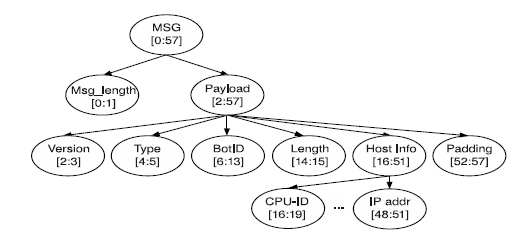
\includegraphics[scale=0.75]{messageformat.jpg}
\caption{Message field tree for the MegaD Host-Information
message}
\label{fig:messageformat}
\end{center}
\end{figure}

\subsection{Field Semantics}
One important property of a field is its semantics, i.e, the type of data that the field contains. Typical field semantics are lengths, timestamps, checksums, hostnames, and filenames. Inferring the field semantics is fundamental to understand what a message does and to identify interesting parts of a dialog to rewrite. Field semantics are captured in the message field tree as an attribute for each field and can be used to label the fields. For example, in Figure\ref{fig:messageformat} the semantics inference states that range [48:51] contains an IP address and range [6:13] contains some data previously received over the network. We use this information to label the corresponding fields \emph{BotID} and \emph{IP addr}.

\subsection{Problem definition}
In this paper we address two problems: 
\begin{enumerate}
\item Extracting the message field tree for the messages \emph{sent} by the application,and 
\item Inferring field semantics, that is, annotating the nodes in the message field tree, for both \emph{received} and \emph{sent} messages, with a field semantics attribute.
\end{enumerate}

\subsection{Approach}
The output buffer contains the message about to be sent at the time that the function that sends data over the network is invoked. As a special case, for encrypted protocols the output buffer contains the unencrypted data at the time the encryption routine is invoked. To extract the format of sent messages we use the following intuition: programs store fields in memory buffers and construct the messages to be sent by combining those buffers together. Thus, the structure of the output buffer represents the inverse of the structure of the sent message. We propose buffer deconstruction, a technique to build the message field tree of a sent message by analyzing how the output buffer is constructed from other memory buffers in the program. We present our message format extraction techniques for sent messages in Section ~\ref{sec:section4} and our handling of encrypted protocols in Section ~\ref{sec:sec5}.

\indent To infer the field semantics, we use type-inference-based techniques that leverage the observation that many functions and instructions used by programs contain known semantic information that can be leveraged for field semantics inference. When a field in the received message is used to derive the arguments of those functions or instructions (i.e., semantic sinks), we can infer its semantics. When the output of those functions or instructions (i.e., semantic sources) are used to derive some field in the output buffer, we can infer its semantics.

\indent We have developed Dispatcher, a tool that enables analyzing both sides of the communication of an unknown protocol, even when an analyst has access only to the application implementing one side of the dialog. Dispatcher integrates previously proposed techniques to extract the message format of received messages, as well as our novel techniques to extract the message format of sent messages, and to infer field semantics in both received and sent messages. We show that the information extracted by Dispatcher enables rewriting MegaD�s C\&C messages.

\subsection{Obtaining an execution trace}
The input to our message format extraction and field semantics inference techniques is execution traces taken by monitoring the program while it is involved in a network dialog using the unknown protocol. To monitor the program we use a custom analysis environment that implements dynamic taint tracking and produces instruction-level execution traces containing all instructions executed, the content of the operands, and the associated taint information. To analyze the protocol used by malware samples (e.g., the C\&C protocol of a botnet) safely, we need to execute them in a specialized analysis network with custom containment policies.

\indent An execution trace contains the processing of multiple messages sent and received by the program during the network dialog. We split the execution trace into per-message traces by monitoring the program�s use of networking functions that read or write data from sockets. We split the execution trace into two traces every time that the program makes a successful call to write data to a socket (e.g., \emph{send}) and every time that the program makes a successful call to read data from a socket (e.g., \emph{recv}), except when the argument defining the maximum number of bytes to read is tainted. In this case, the read data is considered part of the previous message and the trace is not split. This handles the case of a program reading a field conveying the length of the message payload and using this value to read the payload itself.

\subsection{Handling obfuscation}
Our dynamic analysis approach is resilient to obfuscation techniques designed to thwart static analysis such as binary packing and inlining unnecessary instructions. However, a premise of our approach is that we can observe a sample�s processing of the received data in our analysis environment (based on a system emulator). Thus, similar to all dynamic approaches, our approach can be evaded using techniques that detect virtualized or emulated environments. Also, while our techniques work well on MegaD, we expect malware to adapt. Thus, we have designed our techniques to target fundamental properties so that they are as resilient as possible to obfuscation. Nevertheless, the techniques proposed in this paper are not specific to malware analysis and can be used to analyze any unknown or undocumented protocols.

\section{Field Semantics Inference}
In this section we present our technique to identify the field semantics of both received and sent messages.

\indent The intuition behind our type-inference-based techniques is that many functions and instructions used by programs contain rich semantic information. We can leverage this information to infer field semantics by monitoring if received network data is used at a point where the semantics are known, or if data to be sent to the network has been derived from data with known semantics. Such inference is very general and can be used to identify a broad spectrum of field semantics including timestamps, filenames, hostnames, ports, IP addresses, and many others. The semantic information of those functions and instructions is publicly available in their prototypes, which describe their goal as well as the semantics of its inputs and outputs. Function prototypes can be found, for example, at the Microsoft Developer Network or the standard C library documentation. For instructions, one can refer to the system manufacturers� manuals.

\subsection{Techniques}
For received messages, Dispatcher uses taint propagation to monitor if a sequence of bytes from the \emph{received} message is used in the \emph{arguments} of some selected function calls and instructions, for which the system has been provided with the function�s prototype. The sequence of bytes in the received message can then be associated with the semantics of the arguments as defined in the prototype. For example, when a program calls the \emph{connect} function Dispatcher uses the function�s prototype to check if any of the arguments on the stack is tainted. The function�s prototype tells us that the first argument is the socket descriptor, the second one is an address structure that contains the IP address and port of the host to connect to, and the third one is the length of the address structure. If the memory locations that correspond to the IP address to connect to in the address structure are tainted from four bytes in the input, then Dispatcher can infer that those four bytes in the input message (identified by the offset in the taint information) form a field that contains an IP address to connect to. Similarly, if the memory locations that correspond to the port to connect to have been derived from two bytes in the input message, it can identify the position of the port field in the input message.

\indent For sent messages, Dispatcher taints the output of selected functions and instructions using a unique source identifier and offset pair. For each tainted sequence of bytes in the output buffer, Dispatcher identifies from which taint source the sequence of bytes was derived. The semantics of the taint source (return values) are given by the function�s or instruction�s prototype, and can be associated to the sequence of bytes. For example, if a program uses the \emph{rdtsc} x86 instruction, we can leverage the knowledge that it takes no input and returns a 64-bit output representing the current value of the processor�s time-stamp counter, which is placed in registers EDX:EAX [4]. Thus, at the time of execution when the program uses \emph{rdtsc}, Dispatcher taints the EDX and EAX registers with a unique source identifier and offset pair. This pair uniquely labels the taint source to be from \emph{rdtsc}, and the offsets identify each byte in the \emph{rdtsc} stream (offsets 0 through 7 for the first use).

\indent A special case of this technique is \emph{cookie} inference. A cookie represents data from a received message that propagates unchanged to the output buffer (e.g., session identifiers). Thus, a cookie is simultaneously identified in the received and sent messages.

\begin{table}[ht,0.5]
\begin{center}
\begin{tabular}[c]{ | p{4cm} | l | l |}
\hline
Field Semantics & Received & Sent \\ \hline \hline
Cookies & Yes & Yes\\ \hline
IP addresses & Yes & Yes\\ \hline
Error Codes & No & Yes\\ \hline
File data & No & Yes\\ \hline
File Information & No & Yes\\ \hline
Filenames & Yes & Yes\\ \hline
Hash/Checksums & Yes & Yes\\ \hline
Hostnames & Yes & Yes\\ \hline
Host Information & No & Yes \\ \hline
Keyboard input & No & Yes\\ \hline
Keywords & Yes & Yes\\ \hline
Length & Yes & Yes\\ \hline
\end{tabular}

\caption{Field semantics identified by Dispatcher for both received and sent messages. Stored data represents data received over the network and \emph{written} to the filesystem or the Windows registry, as opposed to data \emph{read} from those sources}
\label{tab:semanticinference}
\end{center}
\end{table}

\subsection{Implementation}
To identify field semantics Dispatcher uses an input set of function and instruction prototypes. By default, Dispatcher includes over one hundred functions and a few instructions for which we have already added the prototypes by searching online repositories. To identify new field semantics and their corresponding functions, we  examine the external functions called by the program in the execution trace. Table\ref{tab:semanticinference} shows the field semantics that Dispatcher can infer from received and sent messages using the predefined functions.
\newpage
\section{Extracting Message Format of Sent Packets} \label{sec:section4}
The message field tree captures the hierarchical field structure of the message as well as the field properties encoded in attributes. To extract the message field tree of a sent message we first reverse-engineer the structure of the output message and output a message field tree with no field attributes. Then, we use specific techniques to identify the field attributes, such as how to identify the field boundary (fixed-length, delimiter, length field) and the keywords present in each field.

\begin{figure}[h]
\begin{center}
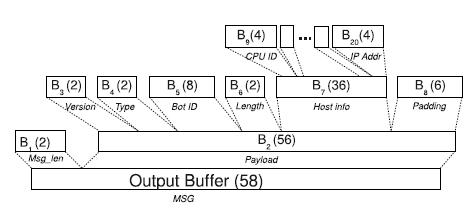
\includegraphics[scale=0.75]{bufferdecon.jpg}
\caption{Buffer deconstruction for the MegaD message in Figure\ref{fig:messageformat}. Each box is a memory buffer starting at address B\textsubscript{x} with the byte length in brackets. Note the similarity with the upsidedown version of Figure\ref{fig:messageformat}}
\end{center}
\label{fig:bufferdecons}
\end{figure}

\indent A field is a sequence of consecutive bytes in a message with some meaning. A memory buffer is a sequence of consecutive bytes in memory that stores data with some meaning. To reverse engineer the structure of the output message we cannot use current techniques to extract the message format of \emph{received} messages because they rely on tainting the network input and monitoring how the tainted data is used by the program. Most data in sent messages does not come from the tainted network input. Instead, we use the following intuition: programs store fields in memory buffers and construct the messages to be sent by combining those buffers together. Thus, the structure of the output buffer represents the inverse of the message field tree of the sent message. We propose \emph{buffer deconstruction}, a technique to build the message field tree of a sent message by analyzing how the output buffer is constructed from other memory buffers in the program. Figure\ref{fig:bufferdecons} shows the deconstruction of the \emph{output buffer} holding the message in Figure\ref{fig:messageformat}. Note the similarity between Figure\ref{fig:messageformat} and the upside-down version of Figure\ref{fig:bufferdecons}.

\indent Extracting the message format of sent messages is a three-step process. In the preparation step, Dispatcher makes a forward pass over the execution trace to extract information about the loops that were executed, the liveness of buffers in the stack, and the call stack information at each point in the execution trace. It also builds an index of the execution trace to enable random access to any instruction. We present the preparation in Section~\ref{sec:4.1}. The core of the message format extraction is the buffer deconstruction step, which is a recursive process in which one memory buffer is deconstructed at a time by extracting the sequence of memory buffers that comprise it. The process is started with the output buffer and recurses until there are no more buffers to deconstruct. Dispatcher implements buffer deconstruction as a backward pass over an execution trace. Since the structure of the output buffer is the inverse of the message field tree for the sent message, every memory buffer that forms the output buffer (and, recursively, the memory buffers that form them) corresponds to a field in the message field tree. For example, deconstructing the output buffer in Figure\ref{fig:bufferdecons} returns a sequence of two buffers, a 2-byte buffer starting at offset zero in the output buffer (B\textsubscript{1}) and a 56-byte buffer starting at offset 2 in the output buffer (B\textsubscript{2}). Correspondingly a field with range [0:1] and another one with range [2:57] are added to the no-attribute message field tree. Thus, buffer deconstruction builds the no-attribute message field tree as it recurses into the output  buffer structure. We present buffer deconstruction in Section~\ref{sec:4.2}. Finally, \emph{field attribute inference} identifies length fields, delimiters, keywords, arrays and variable-length fields and adds the information into attributes for the corresponding fields in the message field tree. We present field attribute inference in Section~\ref{sec:4.3}.

\subsection{Preparation} \label{sec:4.1}

During preparation, Dispatcher makes a forward pass over the execution trace collecting information needed by the buffer deconstruction as well as the attribute inference.

\subsubsection{Loop analysis}
\indent During the forward pass, Dispatcher extracts information about each loop present in the execution trace. To identify the loops in the execution trace, Dispatcher supports two different detection methods: static and dynamic. The static method extracts the addresses of the loop head and exit conditions statically from the binary before the forward pass starts, and uses that information during the forward pass to identify the points where any of those loops appears in the trace. The dynamic method does not require any static processing and extracts the loops directly during the forward pass by monitoring instructions that appear multiple times in the same function. Both methods are complementary. While using static information is more precise at identifying the loop exit conditions, it also requires analyzing all the modules (executable plus dynamically link libraries) used by the application, may miss loops that contain indirection, and cannot be applied if the unpacked binary is not available, such as in the case of MegaD. On the other hand, the dynamic method is less accurate at identifying the loop exit conditions, but requires no setup and can be used on any of our samples including MegaD.

\subsubsection{Callstack Analysis}
\indent During the forward pass, Dispatcher replicates the function stack of the program by monitoring the function calls and returns. Given an instruction number in the execution trace, the callstack analysis returns the innermost function that contained that instruction at that point of the execution.

\subsubsection{Buffer Liveness Analysis}
\indent During the execution trace capture, Dispatcher monitors the heap allocation and free functions used by the program. For each heap allocation it provides the instruction number in the trace, the buffer start and the size of the buffer. For each heap deallocation, it specifies the instruction number in the trace, and the start address of the buffer being freed. During the forward pass, Dispatcher monitors the stack pointer at the function entry and return points, extracting information about which memory locations in the stack are freed when the function returns. This information is used by Dispatcher to determine whether two different writes to the same memory address correspond to the same memory buffer, since memory locations in the stack (and occasionally in the heap) may be reused for different buffers.

\subsection{Buffer Deconstruction} \label{sec:4.2}
Buffer deconstruction is a recursive process. In each iteration it deconstructs a given memory buffer into the sequence of other memory buffers that comprise it. The process starts with the output buffer and recurses until there are no more buffers to deconstruct. It has two parts. First, for each byte in the given buffer we build a \emph{dependency chain}. Then, using the dependency chains and the information collected in the preparation step, we extract the structure of the given buffer. The input to each buffer deconstruction iteration is a buffer defined by its start address in memory, its length, and the instruction number in the trace where the buffer was last written. The start address and length of the output buffer are obtained from the arguments of the function that sends the data over the network (or the encryption function). The instruction number to start the analysis is the instruction number for the first instruction in the send (or encrypt) function. In the remainder of this section we introduce what locations and dependency chains are and present how they are used to deconstruct the output buffer.

\subsubsection{Program locations}
We define a \emph{program location} to be a onebyte-long storage unit in the program�s state. We consider four types of locations: \emph{memory locations, register locations, immediate locations,} and \emph{constant locations}, and focus on the address of those locations, rather than on its content. Each memory byte is a memory location indexed by its address. Each byte in a register is a register location, for example, there are 4 locations in EAX:EAX(0) or AL, EAX(1) or AH, EAX(2), and EAX(3). An immediate location corresponds to a byte from an immediate in the code section of some module, indexed by the offset of the byte with respect to the beginning of the module. Constant locations represent the output of some instructions that have constant output. For example, one common instruction is to XOR one register against itself (e.g.,\emph{ xor \%\thinspace eax, \%\thinspace eax}), which clears the register. Dispatcher recognizes a number of such instructions and makes each byte of its output a constant location.

\subsubsection{Dependency Chains}
A dependency chain for a program location is the sequence of \emph{write operations} that produced the value of the location at a certain point in the program. A write operation comprises the instruction number at which the write occurred, the destination location (i..e, the location that was written), the source location (i.e., the location that was read), and the offset of the written location with respect to the beginning of the output buffer. Figure\ref{fig:depchain} shows the dependency chains for the B\textsubscript{2} buffer (the one that holds the encrypted payload) in Figure\ref{fig:bufferdecons}. In the figure, each box represents a write operation, and each sequence of vertical boxes represents the dependency chain for one location in the buffer.


\begin{figure}[t]
\begin{center}
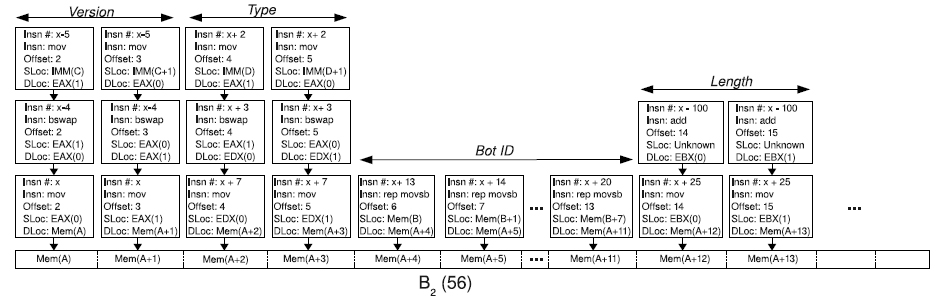
\includegraphics[scale=0.50]{depchain.jpg}
\caption{Dependency chain for B\textsubscript{2} in Figure\ref{fig:bufferdecons}. The start address of B\textsubscript{2} is A.}
\end{center}
\label{fig:depchain}
\end{figure}

\indent The dependency chain is computed in a backward pass starting at the given instruction number. We stop building the dependency chain at the first write operation for which the source location is: 
\begin{enumerate}
\item an immediate location, 
\item a constant location,
\item a memory location,
\item an unknown location
\end{enumerate}

\indent If the source location is part of an immediate or part of the output from some constant output instruction, then there are no more dependencies and the chain is complete. This is the case for the first four bytes of B\textsubscript{2} in Figure\ref{fig:depchain}. The reason to stop at a source memory location is that we want to understand how a memory buf{}fer has been constructed from other memory buf{}fers. After extracting the structure of the given buf{}fer, Dispatcher recurses on the buf{}fers that form it. For example, in Figure\ref{fig:depchain} the dependency chains for locations \emph{Mem(A+4)} through \emph{Mem(A+11)} contains only one write operation because the source location is another memory location. Dispatcher will then create a new dependency chain for buf{}fer \emph{Mem(B)} through \emph{Mem(B+7)}. When building the dependency chains, Dispatcher only handles a small subset of x86 instructions which simply move data around, without modifying it. This subset includes move instructions (\texttt {mov,movs}), move with zero-extend instructions (\texttt{movz}), push and pop instructions, string stores (\texttt{stos}), and instructions that are used to convert data from network to host order and vice versa such as exchange instructions (\texttt{xchg}), swap instructions (\texttt{bswap}), or right shifts that shift entire bytes (e.g.,{\tt shr \$0x8,\%\thinspace eax}). When a write operation is performed by any other instruction, the source is considered unknown and the dependency chain stops. Often, it is enough to stop the dependency chain at such instructions, because the program is at that point performing some operation on the field (e.g., an arithmetic operation) as opposed to just moving the content around. Since programs operate on leaf fields, not on hierarchical f{}ields, then at that point of the chain we have already recursed up to the corresponding leaf f{}ield in the message f{}ield tree. For example, in Figure\ref{fig:depchain} the dependency chains for the last two bytes stop at the same \texttt{add} instruction. Thus, both source locations are unknown. Note that those locations correspond to the length field in Figure\ref{fig:messageformat}. The fact that the program is increasing the length value indicates that the dependency chain has already reached a leaf field.

\subsubsection{Extracting the buffer structure}
We call the source location of the last element in the dependency chain of a buf{}fer location its \emph{source}. We say that two source locations belong to the same source buf{}fer if they are contiguous memory locations (in either ascending or descending order) and the liveness information states that none of those locations has been freed between their corresponding write operations. If the source locations are not in memory (e.g., register, immediate, constant or unknown location), they belong to the same buffer if they were written by the same instruction (i.e, same instruction number).

\indent To extract the structure for the given buf{}fer Dispatcher iterates on the buffer locations from the buf{}fer start to the buf{}fer end. For each buf{}fer location, Dispatcher checks whether the source of the current buf{}fer location belongs to the same source buf{}fer as the source of the previous buf{}fer location. If they do not, then it has found a boundary in the structure of the buf{}fer. The structure of the given buf{}fer is output as a sequence of ranges that form it, where each range states whether it corresponds to a source memory buf{}fer.

\indent For example, in Figure\ref{fig:depchain} the source locations for \emph{Mem(A+4)} and \emph{Mem(A+5)} are contiguous locations \emph{Mem(B)} and \emph{Mem(B+1)} but the source locations for \emph{Mem(A+11)} and \emph{Mem(A+12)} are not contiguous. Thus, Dispatcher marks location \emph{Mem(A+12)} as the beginning of a new range. Dispatcher finds 6 ranges in B\textsubscript{2}. The first four are shown in Figure\ref{fig:depchain} and marked with arrows at the top of the figure. Since only the third range originates from another memory buf{}fer, that is the only buf{}fer that Dispatcher will recurse on to reconstruct. The last two ranges correspond to the Host Info field and the padding in Figure\ref{fig:messageformat} and are not shown in Figure\ref{fig:depchain}.

\indent Once the buf{}fer structure has been extracted, Dispatcher uses the correspondence between buf{}fers and fields in the analyzed message to add one field to the message field tree per range in the buf{}fer structure using the offsets relative to the output buf{}fer. In Figure\ref{fig:depchain} it adds four new fields that correspond to the \emph{Version, Type, Bot ID,} and \emph{Length} in Figure\ref{fig:messageformat}.

\subsection{Field Attribute Inference} \label{sec:4.3}
The message field tree built during the buf{}fer deconstruction step represents the hierarchical structure of the output message, but does not contain information about inter-field relationships such as if a field represents the length of another target field. Such additional information is captured by the field attributes in the message field tree.

\begin{table}[ht,0.5]
\begin{center}
\begin{tabular}[c]{| l | l |}
\hline
Attribute & Value \\ \hline
Field Range & Start offset and length in message\\ \hline
Field Boundary & Fixed,Length and Delimiter\\ \hline
Field Semantics & A value from Table\ref{tab:semanticinference} \\ \hline
Field Keywords & List of keywords in field\\ \hline
%\caption{Field attributes used in the message field tree}
\end{tabular}
\end{center}
\caption{Field attributes used in the message field tree}
\label{tab:fieldattri}
\end{table}

\indent Table\ref{tab:fieldattri} presents the field attributes that we identify in this paper. The field range captures the position of the field in the message. The field boundary captures how an application determines where the field ends. Fields can be fixed-length (\emph{Fixed}), variable-length using a length field (\emph{Length}), or variable-length using a delimiter (\emph{Delimiter}). The field semantics are the values in Table\ref{tab:semanticinference}. The field keywords attribute contains a list of all the protocol constants that appear in the field and their position.

\indent The field attributes in Table\ref{tab:fieldattri} are similar to the ones that previous work extracts for received messages [18, 49]. However, these techniques do not work on sent messages because they rely on monitoring how the data received over the network is processed, when for sent messages we can only observe how the sent messages are built. Our techniques share common intuitions with previous techniques: both try to capture the fundamental properties of the different protocol elements. In fact, some attribute values are more difficult to extract for sent messages than for received messages. For example, many fields that a protocol specification would define as variable length may encode some fixed-length data in a specific implementation. For example the \emph{Server} header is variable-length based on the HTTP specification. However, a given HTTP server implementation may have hard-coded the \emph{Server} string in the binary, making the field fixed-length for this implementation. Leveraging the availability of multiple implementations of the same protocol could help in such cases. We plan to study this in future work.

\subsubsection{Keywords}
Keywords are constants that appear in network messages. To identify constants in the output buffer, Dispatcher taints the memory region that contains the module (and DLLs shipped with the main binary) with a specific taint source, effectively tainting both immediates in the code section as well as data stored in the data section. Locations in the output buffer tainted from this source are considered keywords.

\subsubsection{Length fields} 
Dispatcher uses three different techniques to identify length fields in \emph{sent} messages. The intuition behind the techniques is that length fields can be computed either by incrementing a counter as the program iterates on the field, or by subtracting pointers to the beginning and the end of the buffer. The intuition behind the first two techniques is that those arithmetic operations translate into an unknown source at the end of the dependency chains for the buffer locations corresponding to the length field. When a dependency chain ends in an unknown source, Dispatcher checks whether the instruction that performs the write is inside a known function that computes the length of a string (e.g., \emph{strlen}) or is a subtraction of pointers to the beginning and end of the buffer. The third technique tries to identify counter increments that do not correspond to well-known string length functions. For each buffer it uses the loop information to identify if most writes to the buffer belong to the same loop. If they do, then it uses the techniques in to extract the loop induction variables. For each induction variable it computes the dependency chain and checks whether it intersects the dependency chains from any output buffer locations that precede the locations written in the loop (since a length field always has to precede its target field). Any intersecting location is part of the length field for the field processed in the loop.

\subsubsection{Delimiters}
Delimiters are constants used by protocols to mark the boundary of variable-length fields. Thus, it is difficult to differentiate a delimiter from any another constant in the output message. To identify delimiters, Dispatcher looks for constants that appear multiple times in the same message or appear at the end of multiple messages in the same session (three appearances are required). Constants can be identified by checking the offsets of the taint information for keyword identification. If the delimiters come from the data section, they can also be identified by checking whether the source address of all instances of the constant comes from the same buffer.

\subsubsection{Variable-length fields} 
Dispatcher marks fields that precede a delimiter, and target fields for previously identified length fields as variable-length fields. It also marks as variable-length fields derived from semantic sources that are known to have variable length such as file data. All others are marked as fixed-length.

\subsubsection{Arrays}
The intuition behind identifying arrays of records is that they are written in loops, one record at a time. Dispatcher uses the loop information extracted during preparation to identify loops that write multiple consecutive fields. Then, it adds to the message field 
tree one \emph{Array} field with the range being the combined range of all the consecutive fields written in the loop, and one \emph{Record} field per range of bytes written in each iteration of the loop.

\section{Handling Encrypted Messages} \label{sec:sec5}
Similar to previous work, our protocol reverse engineering techniques work on unencrypted data. Thus, when reverse-engineering encrypted protocols we need to address two problems. First, for received messages, we need to identify the buffers holding the unencrypted data at the point that the decryption has finished since buffers may only hold the decrypted data for a brief period of time. Second, for sent messages, we need to identify the buffers holding the unencrypted data at the point that the encryption is about to begin. Once the buffers holding the unencrypted data have been identified, protocol reverse engineering techniques can be applied on them, rather than on the messages received or about to be sent on the wire.

\indent Recent work has looked at the problem of reverse-engineering the format of received encrypted messages [39, 48]. Since the application needs to decrypt the data before using it, those approaches monitor the application�s processing of the encrypted message and attempt to locate the buffers that contain the decrypted data at the point that the decryption has finished. Those approaches do not address the problem of finding the buffers holding the unencrypted data before it is encrypted, which is also required in our case.

\indent In this work we present two extensions to the technique presented in ReFormat [48]. First, ReFormat can only handle applications where there exists a single boundary between decryption and normal protocol processing. However, multiple such boundaries may exist. As shown in Figure 1 MegaD messages comprise two bytes with the message length, followed by the encrypted payload. After checking the message length, a MegaD bot will decrypt 8 bytes from the encrypted payload and process them, then move to the next 8 bytes and process them, and so on. In addition, some messages in MegaD also use compression and the decryption and decompression operations are interleaved. Thus, there is no single program point where all data in a message is available unencrypted and uncompressed. Consequently, we extend the technique to identify every \emph{instance} of encryption, hashing, compression, and obfuscation, which we generally term \emph{encoding functions}. Second, ReFormat was not designed to identify the buffers holding the unencoded (unencrypted) data before encoding (encryption). Thus, we extend the technique to also cover this case. We present the generalized technique next.

\subsection{Identifying encoding functions}
To identify every instance of an encoding function we have simplified the process in ReFormat by removing the cumulative metric, the use of tainted data, and the concept of leaf functions. The extended technique applies the intuition in ReFormat that the decryption process contains an inordinate number of arithmetic and bitwise operations to encoding functions. It works as follows. Dispatcher makes a forward pass over the input execution trace replicating the callstack of the application by monitoring the call and return instructions. For each function it computes the ratio between the number of arithmetic and bitwise operations over the total number of instructions in the function. The ratio includes only the function�s own instructions. It does not include instructions belonging to any invoked subfunctions. The ratio is computed for each appearance of the function in the trace. Any function that executes a minimum number of instructions and has a ratio larger than a pre-defined threshold is flagged by Dispatcher as an instance of a encoding function. In our experiments, the threshold is set to 0.55 and the minimum number of instructions is 20. Our evaluation results in Section~\ref{sec:6.3} show that the generalized technique identifies all instances of the decryption and encryption functions in our MegaD traces and that the false positive rate of the technique is 0.002\%.

\subsection{Identifying the buffers}
To identify the buffers holding the unencrypted data before encryption we compute the \emph{read set} for the encryption routine, the set of locations read inside the encryption routine before being written. The read set for the encryption routine includes the buffers holding the unencrypted data, the encryption key, and any hard-coded tables used by the routine. We can differentiate the buffers holding the unencrypted data because their content varies between multiple instances of the same function. To identify the buffers holding the unencrypted data after decryption we compute the \emph{write set} for the decryption routine, the set of locations written inside the decryption routine and read later in the trace.

\section{Evaluation}
In this section we evaluate our techniques on the MegaD C\&C protocol, as well as a number of open protocols.

\subsection{Evaluation on MegaD}
MegaD uses a proprietary, encrypted, binary protocol previously not understood. Our MegaD evaluation has two parts. We first describe the information obtained by Dispatcher on the C\&C protocol used by MegaD, and then show how the information extracted by Dispatcher can be used to rewrite a C\&C dialog.


\subsubsection{MegaD C\&C Protocol}
The MegaD C\&C protocol uses port 443 over TCP for transport, employing a proprietary encryption algorithm instead of the SSL routines for HTTPS commonly used on that port. Our network traces show our MegaD bot communicating with three entities: the C\&C server that the bot periodically probes for new commands; the SMTP test server, an SMTP server whose 
hostname is provided by the C\&C server and to which the bot connects to test for spam sending capabilities; and the spam server, whose IP address and listening port are sent by the C\&C server to the bot so that the bot can download all spam-related information such as the spam template or the email addresses to spam. Communication with the C\&C and spam servers uses the encrypted C\&C protocol, while communication with the SMTP test server uses unencrypted SMTP. The communication model is pull-based. The bot periodically probes the botmaster by sending a request message. The botmaster replies with two messages: one with authentication information, and the other one with a command. The bot performs the requested action and sends a response with its results. 

\subsubsection{Message format}
Our MegaD C\&C traces contain 15 different messages (7 received and 8 sent by the bot). Using Dispatcher, we have extracted the message field tree for messages on both directions, as well as the associated field semantics. All 15 messages follow the structure shown in Figure\ref{fig:messageformat} with a 2-byte message length followed by an encrypted payload. The payload, once decrypted,contains a 2-byte field that we term version as it is always a keyword of value 0x100 or 0x1, followed by a 2-byte message type 
field. The structure of the remaining payload depends on the message type. To summarize  the protocol format we have used the output of Dispatcher to write a BinPac grammar that comprises all 15 messages. Field semantics are added as comments to the grammar.

\indent To the best of our knowledge, we are the first to document the C\&C protocol employed by MegaD. Thus, we lack ground truth to evaluate our grammar. To verify the grammar�s accuracy, we use another execution trace that contains a different instance of one of the analyzed dialogs. We dump the content of all unencrypted messages and try to parse the messages using our grammar. For this, we employed a stand-alone version of the BinPac parser included in Bro. Using our grammar, the parser successfully parses all MegaD C\&C messages in the new dialog. In addition, the parser throws an error when given messages that do not follow the MegaD grammar.

\subsubsection{Attribute detection}
The 15 MegaD messages contain no delimiters or arrays. They contain two variable-length fields that use length fields to mark their boundaries: the compressed spam-related information (i.e., template and addresses) received from the spam server, and the host information field in Figure\ref{fig:messageformat}. Both the length fields and variable-length fields are correctly detected by Dispatcher. The only attributes that Dispatcher misses are the message length fields on sent messages because they are computed using complex pointer arithmetic that Dispatcher cannot reason about.

\subsubsection{Field semantics}
Dispatcher identifies 11 different field semantics over the 15 messages: IP addresses, ports, hostnames, length, sleep timers, error codes, keywords, cookies, stored data, padding and host information. There are only two fields in the MegaD grammar for which Dispatcher does not identify their semantics. Both of them happen in received messages: one of them is the message type, which we identify by looking for fields that are compared
against multiple constants in the execution and for which the message format varies depending on its value. The other corresponds to an integer whose value is checked by the program but apparently not used further. Note that we identify some fields in sent messages as keywords because they come from immediates and constants in the data section. We cannot identify exactly what they represent because we do not see how they are used by the C\&C server.

\subsubsection{Rewriting a MegaD dialog}
To show how our grammar enables live rewriting, we run a live MegaD bot inside our analysis environment, which is located in a network that filters all outgoing SMTP connections for containment purposes. In a first dialog, the C\&C server sends the command to the bot ordering to test for spam capability using a given Spam test server. The analysis network blocks the SMTP connection causing the bot to send an error message back to the C\&C server, to communicate that it cannot send spam. No more spam-related messages are received by the bot. Then, we start a new dialog where at the time the bot calls the encrypt function to encrypt the error message, we stop the execution, rewrite the encryption buffer with the message that indicates success, and let the execution continue. After the rewriting the bot keeps receiving the spam-related messages, including the spam template and the addresses to spam, despite the fact that it cannot send any spam messages. Note that simply replaying the message that indicates success from a previous dialog into the new dialog does not work because the success message includes a cookie value that the C\&C selects and may change between dialogs.

\begin{sidewaystable}
\caption{Comparison of the message field tree for sent messages extracted by Dispatcher and Wireshark}
\vspace{0.5cm}
\begin{singlespace}
\label{tab:comparmft}

\begin{tabular}{|c|c|c|c|c|c|c|c|c|c|}
\hline 
\multicolumn{1}{|c}{} &  & \multicolumn{1}{c}{Wireshark} &  & \multicolumn{1}{c}{Dispatcher} &  & \multicolumn{1}{c}{} & \multicolumn{1}{c}{Errors} & \multicolumn{1}{c}{} & \tabularnewline
\hline
\hline 
Protocol & Message Type & \textbar L$_{\text{W}}$ \textbar & \textbar H$_{\text{}W}$ \textbar & \multicolumn{1}{c|}{\textbar L$_{\text{D}}$ \textbar} & \textbar H$_{\text{D}}$ \textbar  & \textbar E(L$_{\text{W}}$) \textbar & \textbar E(L$_{\text{D}}$) \textbar & \textbar E(H$_{\text{}W}$) \textbar & \textbar E(H$_{\text{D}}$) \textbar\tabularnewline
\hline 
HTTP & GET reply & 11 & 1 & 22 & 0 & 11 & 1 & 0 & 1\tabularnewline
\cline{2-10} 
 & POST reply & 11 & 1 & 22 & 0 & 11 & 1 & 0 & 1\tabularnewline
\hline 
DNS & A reply & 27 & 4 & 28 & 0 & 1 & 0 & 0 & 4\tabularnewline
\hline 
FTP & Welcome0 & 2 & 1 & 3 & 1 & 1 & 0 & 0 & 0\tabularnewline
\cline{2-10} 
 & Welcome1 & 2 & 1 & 3 & 1 & 1 & 0 & 0 & 0\tabularnewline
\cline{2-10} 
 & Welcome2 & 2 & 1 & 3 & 1 & 1 & 0 & 0 & 0\tabularnewline
\cline{2-10} 
 & USER reply & 2 & 1 & 3 & 1 & 1 & 1 & 0 & 0\tabularnewline
\cline{2-10} 
 & PASS reply & 2 & 1 & 2 & 0 & 1 & 1 & 0 & 1\tabularnewline
\cline{2-10} 
 & SYST reply & 2 & 1 & 2 & 0 & 1 & 1 & 0 & 1\tabularnewline
\hline 
ICQ & New Connection & 5 & 0 & 5 & 0 & 0 & 0 & 0 & 0\tabularnewline
\cline{2-10} 
 & AIM sign-on & 11 & 3 & 15 & 3 & 5 & 0 & 0 & 0\tabularnewline
\cline{2-10} 
 & AIM log-on & 46 & 15 & 46 & 15 & 0 & 0 & 0 & 0\tabularnewline
\hline 
\multicolumn{1}{|c}{Total} &  & 123 & 30 & 154 & 22 & 34 & 5 & 0 & 8\tabularnewline
\hline
\end{tabular}


\end{singlespace}
\end{sidewaystable}

\subsection{Evaluation on Open Protocols}
In this section we evaluate our techniques on four open protocols: HTTP , DNS, FTP, and ICQ. To this end, we compare the output of Dispatcher with that of Wireshark 1.0.5 [12] when processing 12 messages belonging to those protocols. For each protocol we select a representative application that implements the protocol: Apache-2.2.1 for HTTP, Bind-9.6.0 for DNS, Filezilla-0.9.31 for FTP, and Pidgin-2.5.5 for ICQ. Note that regardless of the application being a client (Pidgin) or a server (Bind, Apache, Filezilla), for this part of the evaluation we focus on sent messages.

\subsubsection{Message format}
Wireshark is a network protocol analyzer containing manually written grammars (called dissectors) for a large variety of network protocols. Although Wireshark is a mature and widely-used tool, its dissectors have been manually generated and therefore are not completely error-free. To compare the accuracy of the message format automatically extracted by Dispatcher to the manually written ones included in Wireshark, we analyze the message field tree output by both tools and manually compare them to the protocol specification. Thus, we can classify any differences between the output of both tools to be due to errors in Dispatcher, Wireshark, or both.

\indent We denote the set of leaf fields and the set of hierarchical fields in the message field tree output by Wireshark as \textbar L$_{\text{W}}$\textbar and \textbar H$_{\text{W}}$\textbar, respectively. \textbar L$_{\text{D}}$\textbar and \textbar H$_{\text{D}}$\textbar are the corresponding sets for Dispatcher. Table\ref{tab:comparmft} shows the evaluation results. For each protocol and message it shows the number of leaf fields and hierarchical fields in the message field tree output by both tools as well as the result of the manual classification of its errors. Here, \textbar L$_{\text{W}}$\textbar and \textbar E(L$_{\text{D}})$\textbar represent the number of errors on leaf fields in the message field tree output by Wireshark and Dispatcher respectively. Similarly, \textbar E(H$_{\text{W}}$)\textbar and \textbar E(H$_{\text{D}}$)\textbar represent the number of errors on hierarchical fields.

\indent The results show that Dispatcher outperforms Wireshark when identifying leaf fields. This surprising result is due to the inconsistencies between the different dissectors in Wireshark when identifying delimiters. Some dissectors do not add delimiter fields to the
message field tree, some concatenate them to the variable-length field for which they mark the boundary, while others treat them as separate fields. After checking the protocol specifications, we believe that delimiters should be treated as their own fields in all
dissectors. The results also show that Wireshark outperforms Dispatcher when identifying hierarchical fields. This is due to the program not using loops to write the arrays because the number of elements in the array is known or is small enough that the compiler has unrolled the loop.

\indent Overall, Dispatcher outperformed Wireshark for the given messages. Note that we do not claim that Dispatcher is generally more accurate than Wireshark since we are only evaluating a limited number of protocols and messages. However, the results show that the accuracy of the message format automatically extracted by Dispatcher can rival that of Wireshark, without requiring a manually generated grammar.

\subsubsection{Errors on leaf fields}
Here we detail the errors on leaf fields that we have assigned to Dispatcher. The error in the HTTP GET reply message is in the Status-Line. The HTTP/1.1 specification states that its format is: \emph{Status-Line = HTTP-Version SP Status-Code SP Reason-Phrase CRLF}, but both Dispatcher and Wireshark consider the Status-Code, the delimiter, and the Reason-Phrase to belong to the same field. The FTP specification states that a reply message comprises a completion code followed by a text string. The error in the FTP USER reply message is due to the fact that the server echoes back the username to the client and Dispatcher identifies the username being echoed back as an additional cookie field. The other FTP replies have the same type of error: the response code is merged with the text string because the program keeps the whole message (except the delimiter) in a single buffer in the data section. As mentioned earlier the errors on hierarchical fields are due to the program being analyzed not using loops to write the arrays. For example, the four errors in the DNS reply correspond to the \emph{Queries, Answers, Authoritative}, and \emph{Additional} sections in the message, which Bind processes separately and therefore Dispatcher cannot identify as an array.

\indent These errors highlight the fact that the message field tree extracted by Dispatcher is limited to the quality of the protocol implementation in the binary, and may differ from the specification.

\subsubsection{Attribute detection}
The 12 messages contain 14 length fields, 43 delimiters, 57 variable-length fields, and 3 arrays. Dispatcher misses 8 length fields because their value is hard-coded in the program.
Thus, their target variable-length fields are considered fixedlength. Out of the 43 delimiters Dispatcher only misses one, which corresponds to a null byte marking the end of a cookie string that was considered part of the string. Dispatcher correctly identifies all other variable-length fields. Out of 3 arrays, Dispatcher misses one formed by the \emph{Queries, Answers, Authoritative}, and \emph{Additional} sections in the DNS reply, which Bind processes separately and therefore cannot be identified by Dispatcher. 

\subsubsection{Field semantics}
Dispatcher correctly identifies all semantic information in the sent messages, except the 3 pointers in the DNS reply, used by the DNS compression method, which are computed using pointer arithmetic that Dispatcher cannot reason about.

\begin{table}
\begin{center}
\begin{tabular}{|c|c|c|c|c|}
\hline
No: of traces & No: of functions & True Positive & False Positive & False Positive Rate\\ \hline
20 & 3,569,773(22,379) & 4,874 & 87(9) & 0.002\% \\ \hline
\end{tabular}
\label{tab:encodstat}
\caption{Evaluation of the detection of encoding functions}
\end{center}
\end{table}

\subsection{Detecting Encoding Function} \label{sec:6.3}
To evaluate the detection of encoding functions presented in Section~\ref{sec:sec5} we perform the following experiment. We obtain 20 execution traces from multiple programs that handle network data. Five
of these traces process encrypted and compressed functions, four of them are from MegaD sessions and the other one is from Apache while handling an HTTPS session. MegaD uses its own encryption algorithm and the \emph{zlib} library for compression and Apache uses SSL with AES and SHA-18. The remaining 15 execution traces are from a variety of programs including browsers (Internet Explorer 7, Safari 3.1, and Google Chrome 1.0), network servers (Bind, Atphttpd), and services embedded in Windows (RPC, MSSQL).

\indent Dispatcher correctly identifies all encoding functions in the execution traces of MegaD and Apache-SSL. In the MegaD traces, all instances of three unique encoding functions are identified: the decryption routine, the encryption routine, and a key generation routine that generates the encryption and decryption keys from a seed value in the binary before calling the encryption or decryption routines. In addition, in the traces that process messages with compressed data, Dispatcher flags a fourth function that corresponds to the \emph{inflate} function in the \emph{zlib} library, which is statically linked into the MegaD binary.

\indent There is a total of 87 false positives from nine unique functions. Of those, we have been able to identify two:{\tt memchr} and {\tt comctl32.dll::TrueSaturateBits}. All instances of the other seven are conservatively classified as false positives. Based on these results, our technique correctly identifies all known encoding functions and has a false positive rate of 0.002\%.

\section{Conclusion}
Automatic protocol reverse-engineering is important for many security applications, including the analysis and infiltration of botnets. Prior techniques cannot enable rewriting of C\&C messages needed for infiltration because they cannot analyze encrypted protocols used by newer botnets, they do not extract information about the semantics of the protocol, or they require access to both peers in a protocol dialog for a complete view of the protocol. In this paper we have addressed those limitations.

\indent We have proposed techniques to extract the message format of sent messages. Our techniques leverage the intuition that the structure of the output buffer represents the inverse of the structure of the sent message. Thus, we introduce buffer deconstruction, a technique that extracts the structure of a message being sent by reconstructing how the output buffer has been built from other memory buffers in the program. In addition, we have proposed techniques for inferring field semantics, a prerequisite for rewriting C\&C messages for botnet infiltration. Our type-inference-based techniques leverage the rich semantic information that is already available in the program by monitoring how data in the received messages is used at places where the semantics are known, and how the sent messages are built from data with known semantics.

\indent We have implemented our techniques as well as previous approaches into Dispatcher, a tool that enables the analysis of protocol dialogs even when only one of the peers involved in the dialog is available. We have used Dispatcher to analyze the previously undocumented C\&C protocol of MegaD, a prevalent spam botnet. We have shown that the information output by Dispatcher enables botnet infiltration by rewriting the C\&C messages

\newpage
\section*{Bibliography}
%\newpage
%\section*{References}
{\bf [1] AMD64 architecture tech docs} \\ \href{http://www.amd.com/}{\tt http://www.amd.com/}\\
{\bf [2] How Samba was written.}\\ \href{http://samba.org/ftp/}{\tt http://samba.org/ftp/}\\
{\bf [3] Icqlib: The ICQ library} \\ \href{http://kicq.sourceforge.net/icqlib.shtml}{\tt http://kicq.sourceforge.net/icqlib.shtml}\\
{\bf [4] Intel64 and IA-32 architectures software developer�s manuals.} \\  \href{http://www.intel.com/products/processor/manuals/}{\tt http://www.intel.com/products/
processor/manuals/.}\\
{\bf [5] The ISO/IEC 9899:1999 C programming language standard} \\ \href{http://www.open-std.org/jtc1/sc22/wg14/www/docs/n1124.pdf}{\tt http://www.open-std.org/jtc1/sc22/wg14/www/docs/n1124.pdf}\\
{\bf [6] Libyahoo2: A C library for Yahoo! Messenger}\\ \href{http://libyahoo2.sourceforge.net.}{\tt http://libyahoo2.sourceforge.net. }\\
{\bf [7] Marshal8e6 security threats: Email and web threats.}\\ \href{http://www.marshal.com/newsimages/trace/Marshal8e6\_TRACE\_Report\_Jan2009.pdf}{\tt http://www.marshal.com/newsimages/trace/Marshal8e6\_TRACE\_Report\_Jan2009.pdf} \\
{\bf [8] MSDN: Microsoft developer network.}\\ \href{http://msdn.microsoft.com}{\tt http://msdn.microsoft.com}\\
{\bf [9] MSN Messenger protocol}\\ \href{http://www.hypothetic.org/docs/msn/index.php}{\tt http://www.hypothetic.org/docs/msn/index.php}\\
{\bf [10] R. Bajcsy, T. Benzel, M. Bishop, B. Braden, C. Brodley, S. Fahmy, S. Floyd, W. Hardaker, A. Joseph, G. Kesidis,K. Levitt, B. Lindell, P. Liu, D. Miller, R. Mundy, C. Neuman, R. Ostrenga, V. Paxson, P. Porras, C. Rosenberg, J. D. Tygar, S. Sastry, D. Sterne, and S. F. Wu, \textquotedblleft Cyber defense technology networking and evaluation,\textquotedblright {\it  Communications of the ACM,} 47(3), 2004. }\\
{\bf [11] M. A. Beddoe. Network protocol analysis using bioinformatics algorithms.}\\ \href{http://www.baselineresearch.net/PI/}{\tt http://www.baselineresearch.net/PI/} \\
{\bf [12] N. Borisov, D. J. Brumley, H. J. Wang, and C. Guo: Generic
application-level protocol analyzer and its language {\it Network and Distributed System Security Symposium,} San Diego, CA, February 2007.}\\
{\bf [13] J. Caballero, H. Yin, Z. Liang, and D. Song. Polyglot: Automatic extraction of protocol message format using dynamic binary analysis. In {\it ACM Conference on Computer and Communications Security} Alexandria, VA, October 2007.}\\
{\bf [14] J. Chow, B. Pfaff, T. Garfinkel, K. Christopher, and M. Rosenblum:Understanding data lifetime via whole system simulation. In {\it USENIX Security Symposium,} San Diego, CA, August 2004}\\
{\bf [15] P. Porras, H. Saidi, and V. Yegneswaran: \textquotedblleft A foray into Conficker�s logic and rendezvous points\textquotedblright. In {\it USENIX Workshop on Large-Scale Exploits and Emergent Threats,} Boston, MA, April 2009.}\\
{\bf [16] C. Leita, M. Dacier, and F. Massicotte : Automatic handling of protocol dependencies and reaction to 0-day attacks with ScriptGen based honeypots. In {\it International Symposium on Recent Advances in Intrusion Detection,} Hamburg, Germany, September 2006.}\\
{\bf [17] G. Wondracek, P. M. Comparetti, C. Kruegel, and E. Kirda: Automatic network protocol analysis. In {\it Network and Distributed System Security Symposium,}San Diego, CA, February 2008.}\\
{\bf G. E. Suh, J. W. Lee, D. Zhang, and S. Devadas: Secure program execution via dynamic information flow tracking. In {\it International Conference on Architectural Support for
Programming Languages and Operating Systems,} Boston, MA, October 2004.}

\addcontentsline{toc}{section}{Bibliography}
\end{onehalfspace}
\end{document}
